% !TeX root = beameruserguide.tex
% Copyright 2003--2007 by Till Tantau
% Copyright 2010 by Vedran Mileti\'c
% Copyright 2013,2015 by Vedran Mileti\'c, Joseph Wright
% Copyright 2016 by Joseph Wright
% Copyright 2017,2018 by Louis Stuart, Joseph Wright
%
% This file may be distributed and/or modified
%
% 1. under the LaTeX Project Public License and/or
% 2. under the GNU Free Documentation License.
%
% See the file doc/licenses/LICENSE for more details.

\section{Creating Frames}
\label{section-frames}


\subsection{The Frame Environment}

A presentation consists of a series of frames. Each frame consists of a series of slides. You create a frame using |frame| environment.\footnote{The command \texttt{\textbackslash frame} is supported for legacy documents.} All of the text that is not tagged by overlay specifications is shown on all slides of the frame. (Overlay specifications are explained in more detail in later sections. For the moment, let's just say that an overlay specification is a list of numbers or number ranges in pointed brackets that is put after certain commands as in |\uncover<1,2>{Text}|.) If a frame contains commands that have an overlay specification, the frame will contain multiple slides; otherwise it contains only one slide.

\begin{environment}{{frame}\sarg{overlay specification}\opt{|[<|\meta{default overlay specification}|>]|}\oarg{options}\opt{\marg{title}\marg{subtitle}}}
  The \meta{overlay specification} dictates which slides of a frame are to be shown. If left out, the number is calculated automatically. The \meta{environment contents} can be normal \LaTeX\ text, but may not contain |\verb| commands or |verbatim| environments or any environment that changes the character codes, unless the |fragile| option is given.

  The optional \meta{title} is detected by an opening brace, that is, if the first thing in the frame is an opening brace then it is assumed that a frame title follows. Likewise, the optional \meta{subtitle} is detected the same way, that is, by an opening brace following the \meta{title}. The title and subtitle can also be given using the |\frametitle| and |\framesubtitle| commands.

  The normal \LaTeX\ command |\frame| is available \emph{inside} frames with its usual meaning. Both outside and inside frames it is always available as {\color{red!75!black}|\framelatex|}.

  \example
\begin{verbatim}
\begin{frame}{A title}
  Some content.
\end{frame}
%% Same effect:
\begin{frame}
  \frametitle{A title}
  Some content.
\end{frame}
\end{verbatim}

  \example
\begin{verbatim}
\begin{frame}<beamer>{Outline}  % frame is only shown in beamer mode
  \tabelofcontent[current]
\end{frame}
\end{verbatim}

  Normally, the complete \meta{environment contents} is put on a slide. If the text does not fit on a slide, being too high, it will be squeezed as much as possible, a warning will be issued, and the text just extends unpleasantly over the bottom. You can use the option |allowframebreaks| to cause the \meta{frame text} to be split among several slides, though you cannot use overlays then. See the explanation of the |allowframebreaks| option for details.

  The \meta{default overlay specification} is an optional argument that is ``detected'' according to the following rule: If the first optional argument in square brackets starts with a |<|, then this argument is a \meta{default overlay specification}, otherwise it is a normal \meta{options} argument. Thus |\begin{frame}[<+->][plain]| would be legal, but also |\begin{frame}[plain]|.

  The effect of the \meta{default overlay specification} is the following: Every command or environment \emph{inside the frame} that accepts an action specification, see Section~\ref{section-action-specifications}, (this includes the |\item| command, the |actionenv| environment, |\action|, and all block environments) and that is not followed by an overlay specification gets the \meta{default overlay specification} as its specification. By providing an incremental specification like |<+->|, see Section~\ref{section-incremental}, this will essentially cause all blocks and all enumerations to be uncovered piece-wise (blocks internally employ action specifications).

  \example
  In this frame, the theorem is shown from the first slide on, the proof from the second slide on, with the first two itemize points shown one after the other; the last itemize point is shown together with the first one. In total, this frame will contain four slides.

\begin{verbatim}
\begin{frame}[<+->]
  \begin{theorem}
    $A = B$.
  \end{theorem}
  \begin{proof}
    \begin{itemize}
    \item Clearly, $A = C$.
    \item As shown earlier,  $C = B$.
    \item<3-> Thus $A = B$.
    \end{itemize}
  \end{proof}
\end{frame}
\end{verbatim}

  The following \meta{options} may be given:
  \begin{itemize}
  \item
    \declare{|allowdisplaybreaks|}\opt{|=|\meta{break desirability}} causes the AMS\TeX\ command |\allowdisplaybreaks|\penalty0|[|\meta{break desirability}|]| to be issued for the current frame. The \meta{break desirability} can be a value between 0 (meaning formulas may never be broken) and 4 (the default, meaning that formulas can be broken anywhere without any penalty). The option is just a convenience and makes sense only together with the |allowsframebreaks| option.
  \item
    \declare{|allowframebreaks|}\opt{|=|\meta{fraction}}. When this option is given, the frame will be automatically broken up into several frames if the text does not fit on a single slide. In detail, when this option is given, the following things happen:
    \begin{enumerate}
    \item
      Overlays are not supported.
    \item
      Any notes for the frame created using the |\note| command will be inserted after the first page of the frame.
    \item
      Any footnotes for the frame will be inserted on the last page of the frame.
    \item
      If there is a frame title, each of the pages will have this frame title, with a special note added indicating which page of the frame that page is. By default, this special note is a Roman number. However, this can be changed using the following template.
      \begin{element}{frametitle continuation}\yes\yes\yes
        The text of this template is inserted at the end of every title of a frame with the |allowframebreaks| option set.
        \begin{templateoptions}
          \itemoption{default}{}
          Installs a Roman number as the template. The number indicates the current page of the frame.

          \itemoption{roman}{}
          Alias for the default.

          \itemoption{from second}{\oarg{text}}
          Installs a template that inserts \meta{text} from the second page of a frame on. By default, the text inserted is |\insertcontinuationtext|,  which  in turn is |(cont.)| by default.
          
          \itemoption{singleframecheck}{\oarg{text}}
          Installs a template that inserts \meta{text} starting from the first page, but only if one or more frame breaks occur in the frame. By default, the text inserted is  |\insertcontinuationcountroman|,  which  will show the continuation count as Roman number.
        \end{templateoptions}
        The following inserts are available:
        \begin{templateinserts}
          \iteminsert{\insertcontinuationcount}
          inserts the current page of the frame as an arabic number.
          \iteminsert{\insertcontinuationcountroman}
          inserts the current page of the frame as an (uppercase) Roman number.
          \iteminsert{\insertcontinuationtext}
          just inserts the text |(cont.)| or, possibly, a translation thereof (like |(Forts.)| in German).
        \end{templateinserts}
      \end{element}
    \end{enumerate}

    If a frame needs to be broken into several pages, the material on all but the last page fills only 95\% of each page by default. Thus, there will be some space left at the top and/or bottom, depending on the vertical placement option for the frame. This yields a better visual result than a 100\% filling, which typically looks crowded. However, you can change this percentage using the optional argument \meta{fraction}, where 1 means 100\% and 0.5 means 50\%. This percentage includes the frame title. Thus, in order to split a frame ``roughly in half,'' you should give 0.6 as \meta{fraction}.

    Most of the fine details of normal \TeX\ page breaking also apply to this option. For example, when you wish equations to be broken automatically, be sure to use the |\allowdisplaybreaks| command. You can insert |\break|, |\nobreak|, and |\penalty| commands to control where breaks should occur. The commands |\pagebreak| and |\nopagebreak| also work, including their options. Since you typically do not want page breaks for the frame to apply also to the |article| mode, you can add a mode specification like |<presentation>| to make these commands apply only to the presentation modes. The command \declare{|\string\framebreak|} is a shorthand for |\pagebreak<presentation>| and \declare{|\string\noframebreak|} is a shorthand for |\nopagebreak<presentation>|.

    The use of this option is \emph{evil}. In a (good) presentation you prepare each slide carefully and think twice before putting something on a certain slide rather than on some different slide. Using the |allowframebreaks| option invites the creation of horrible, endless presentations that resemble more a ``paper projected on the wall'' than a presentation. Nevertheless, the option does have its uses. Most noticeably, it can be convenient for automatically splitting bibliographies or long equations.

    \example
\begin{verbatim}
\begin{frame}[allowframebreaks]{References}
  \begin{thebibliography}{XX}

  \bibitem...
  \bibitem...
    ...
  \bibitem...
  \end{thebibliography}
\end{frame}
\end{verbatim}

    \example
\begin{verbatim}
\begin{frame}[allowframebreaks,allowdisplaybreaks]{A Long Equation}
  \begin{align}
    \zeta(2) &= 1 + 1/4 + 1/9 + \cdots \\
    &= ... \\
    ...
    &= \pi^2/6.
  \end{align}
\end{frame}
\end{verbatim}

  \item
    \declare{|b|}, \declare{|c|}, \declare{|t|} will cause the frame to be vertically aligned at the bottom/center/top. This overrides the global placement policy, which is governed by the class options |t| and |c|.
  \item
    \declare{|s|} will cause the content of the frame to be distributed vertically across the whole frame. For a reasonable usage of the option, the user has to add ``stretchable'' material to the frame content, e.g. |\vfill| or similar macros.
  \item
    \declare{|noframenumbering|} tells \beamer\ not to step the |framenumber| counter for this frame.
  \item
    \declare{|fragile|\opt{|=singleslide|}} tells \beamer\ that the frame contents is ``fragile.'' This means that the frame contains text that is not ``interpreted as usual.'' For example, this applies to verbatim text, which is, obviously, interpreted somewhat differently from normal text.

    If a frame contains fragile text, different internal mechanisms are used to typeset the frame to ensure that inside the frame the character codes can be reset. The price of switching to another internal mechanism is that either you cannot use overlays or an external file needs to be written and read back (which is not always desirable).

    In detail, the following happens when this option is given for normal (pdf)\LaTeX: The contents of the frame is scanned and then written to a special file named \meta{jobname}|.vrb| or, if a label has been assigned to the frame, \meta{jobname}|.|\meta{current frame number}|.vrb|. Then, the frame is started anew and the content of this file is read back. Since, upon reading of a file, the character codes can be modified, this allows you to use both verbatim text and overlays.

    To determine the end of the frame, the following rule is used: The first occurrence of a single line containing exactly |\end{|\meta{frame environment name}|}| ends the frame. The \meta{environment name} is normally |frame|, but it can be changed using the |environment| option. This special rule is needed since the frame contents is, after all, not interpreted when it is gathered.

    You can also add the optional information |=singleslide|. This tells \beamer\ that the frame contains only a single slide. In this case, the frame contents is \emph{not} written to a special file, but interpreted directly, which is ``faster and cleaner.''
  \item
    \declare{|environment=|\meta{frame environment name}}. This option is useful only in conjunction with the |fragile| option (but it is not used for |fragile=singleslide|, only for the plain |fragile|). The \meta{frame environment name} is used to determine the end of the scanning when gathering the frame contents. Normally, the frame ends when a line reading |\end{frame}| is reached. However, if you use |\begin{frame}| inside another environment, you need to use this option:

    \example
\begin{verbatim}
\newenvironment{slide}[1]
  {\begin{frame}[fragile,environment=slide]
      \frametitle{#1}}
  {\end{frame}}

\begin{slide}{My title}
  Text.
\end{slide}
\end{verbatim}

    If you did not specify the option |environment=slide| in the above example, \TeX\ would ``miss'' the end of the slide since it does not interpret text while gathering the frame contents.
  \item
    \declare{|label=|\meta{name}} causes the frame's contents to be stored under the name \meta{name} for later resumption using the command |\againframe|. Furthermore, on each slide of the frame a label with the name \meta{name}|<|\meta{slide number}|>| is created. On the \emph{first} slide, furthermore, a label with the name \meta{name} is created (so the labels \meta{name} and \meta{name}|<1>| point to the same slide). Note that labels in general, and these labels in particular, can be used as targets for hyperlinks.

    You can use this option together with |fragile|.
  \item
    \declare{|plain|} causes the headlines, footlines, and sidebars to be suppressed. This is useful for creating single frames with different head- and footlines or for creating frames showing big pictures that completely fill the frame.

    \example
    A frame with a picture completely filling the frame:

\begin{verbatim}
\begin{frame}[plain]
  \begin{centering}%
    \pgfimage[height=\paperheight]{somebigimagefile}%
    \par%
  \end{centering}%
\end{frame}
\end{verbatim}

    \example
    A title page, in which the head- and footlines are replaced by two graphics.

\begin{verbatim}
\setbeamertemplate{title page}
{
  \pgfuseimage{toptitle}
  \vskip0pt plus 1filll

  \begin{centering}
    {\usebeamerfont{title}\usebeamercolor[fg]{title}\inserttitle}

    \insertdate
  \end{centering}

  \vskip0pt plus 1filll
  \pgfuseimage{bottomtitle}
}
\begin{frame}[plain]
  \titlepage
\end{frame}
\end{verbatim}

  \item
    \declare{|shrink|}\opt{|=|\meta{minimum shrink percentage}}. This option will cause the text of the frame to be shrunk if it is too large to fit on the frame. \beamer\ will first normally typeset the whole frame. Then it has a look at vertical size of the frame text (excluding the frame title). If this vertical size is larger than the text height minus the frame title height, \beamer\ computes a shrink factor and scales down the frame text by this factor such that the frame text then fills the frame completely. Using this option will automatically cause the |squeeze| option to be used, also.

    Since the shrinking takes place only after everything has been typeset, shrunk frame text will not fill the frame completely horizontally. For this reason, you can specify a \meta{minimum shrink percentage} like |20|. If this percentage is specified, the frame will be shrunk \emph{at least} by this percentage. Since \beamer\ knows this, it can increase the horizontal width proportionally such that the shrunk text once more fills the entire frame. If, however, the percentage is not enough, the text will be shrunk as needed and you will be punished with a warning message.

    The best way to use this option is to identify frames that are overly full, but in which all text absolutely has to be fit on a single frame. Then start specifying first |shrink=5|, then |shrink=10|, and so on, until no warning is issued any more (or just ignore the warning when things look satisfactory).

    Using this option is \emph{very evil}. It will result in changes of the font size from slide to slide, which is a typographic nightmare. Its usage can \emph{always} be avoided by restructuring and simplifying frames, which will result in a better presentation.

    \example
\begin{verbatim}
\begin{frame}[shrink=5]
  Some evil endless slide that is 5\% too large.
\end{frame}
\end{verbatim}

  \item
    \declare{|squeeze|} causes all vertical spaces in the text to be squeezed together as much as possible. Currently, this just causes the vertical space in enumerations or itemizations to be reduced to zero.

    Using this option is not good, but also not evil.
  \end{itemize}

  \articlenote
  In |article| mode, the |frame| environment does not create any visual reference to the original frame (no frame is drawn). Rather, the frame text is inserted into the normal text. To change this, you can modify the templates |frame begin| and |frame end|, see below. To suppress a frame in |article| mode, you can, for example, specify |<presentation>| as overlay specification.

  \begin{element}{frame begin}\yes\no\no
    The text of this template is inserted at the beginning of each frame in |article| mode (and only there). You can use it, say, to start a |minipage| environment at the beginning of a frame or to insert a horizontal bar or whatever.
  \end{element}

  \begin{element}{frame end}\yes\no\no
    The text of this template is inserted at the end of each frame in |article| mode.
  \end{element}
\end{environment}

You \emph{can} use the |frame| environment inside other environments like this

\begin{verbatim}
\newenvironment{slide}{\begin{frame}}{\end{frame}}
\end{verbatim}

or like this

\begin{verbatim}
\newenvironment{myframe}[1]
  {\begin{frame}[fragile,environment=myframe]\frametitle{#1}}
  {\end{frame}}
\end{verbatim}

However, the actual mechanics are somewhat sensitive since the ``collecting'' of the frame contents is not easy, so do not attempt anything too fancy. As a rule, the beginning of the environment can be pretty arbitrary, but the ending must end with |\end{frame}| and should not contain any |\end{xxx}|. Anything really complex is likely to fail. If you need some |\end{xxx}| there, define a new command that contains this stuff as in the following example:

\begin{verbatim}
\newenvironment{itemizeframe}
  {\begin{frame}\startitemizeframe}
  {\stopitemizeframe\end{frame}}

\newcommand\startitemizeframe{\begin{bfseries}\begin{itemize}}
\newcommand\stopitemizeframe{\end{itemize}\end{bfseries}}

\begin{itemizeframe}
\item First item
\end{itemizeframe}
\end{verbatim}


\subsection{Components of a Frame}

Each frame consists of several components:
\begin{enumerate}\itemsep=0pt\parskip=0pt
\item a headline and a footline,
\item a left and a right sidebar,
\item navigation bars,
\item navigation symbols,
\item a logo,
\item a frame title,
\item a background, and
\item some frame contents.
\end{enumerate}

A frame need not have all of these components. Usually, the first three components are automatically setup by the theme you are using. 
Figure \ref{fig:framelayers} shows an overview of the order in which the different components are drawn.

\begin{figure}[htbp]
% the following code is based on https://gist.githubusercontent.com/loopspace/c37dd788b217f2e963587278c3532f73/raw/f6e4708f36f661193ea7aed3cba7d389226658cc/beamerframe.tex
\begin{tikzpicture}[z={(0.97,0)},x={(.55,.4)}]

% colour palette generated by mycolor.space to match beamer's beamer@blendedblue
\definecolor{fc_col1}{HTML}{3333b3}
\definecolor{fc_col2}{HTML}{b1a3d9}
\definecolor{fc_col3}{HTML}{fffade}
\definecolor{fc_col4}{HTML}{68baa5}
\definecolor{fc_col5}{HTML}{ae0000}

\colorlet{base}{fc_col3}
\colorlet{background canvas}{base}
\colorlet{logo bg}{fc_col1}
\colorlet{sidebar left}{fc_col4}
\colorlet{sidebar right}{fc_col4}
\colorlet{section in sidebar}{fc_col5}
\colorlet{logo fg}{white}
\colorlet{footline}{fc_col2}
\colorlet{navigation symbols}{fc_col1}

\pgfmathsetmacro{\bepgw}{12.8}
\pgfmathsetmacro{\bepgh}{9.6}
\newcommand{\component}[3][1]{%
\path (#2) [draw,<-,thick] -- (#2 |- 0,-\bepgh-#1,0) node[below,text width=2cm,align=center] (#3) {#3};
\stepcounter{zlayer}}
\newcounter{zlayer}
\setcounter{zlayer}{0}
\def\zlayer{\the\value{zlayer}}

\foreach \z in {0,...,10} {
  \draw[gray,ultra thick] (0,-\bepgh,\z) -- (\bepgw,-\bepgh,\z) -- (\bepgw,0,\z);
}

% background canvas
\fill[background canvas] (0,0,\zlayer) -- ++(\bepgw,0,0) -- ++(0,-\bepgh,0) -- ++(-\bepgw,0,0) -- cycle;
\component[1]{1,-\bepgh,\zlayer}{background canvas}

% background
\draw[gray] \foreach \x in {0,...,\bepgw} \foreach \y in {0,...,\bepgh} {(\x,0,\zlayer) -- (\x,-\bepgh,\zlayer) (0,-\y,\zlayer) -- (\bepgw,-\y,\zlayer)};
\component[2]{1,-\bepgh,\zlayer}{background}

% left sidebar
\fill[sidebar left] (0,0,\zlayer) -- ++(2,0,0) -- ++(0,-\bepgh,0) -- ++(-2,0,0) -- cycle;
\component[3]{1,-\bepgh,\zlayer}{sidebar canvas left}

% section in sidebar
\node[yslant=.7,right,align=left,text=section in sidebar,font=\sffamily] at (0,-.45*\bepgh,\zlayer) (a section in sidebar) {First slide \\ Second slide \\ Third slide};
\component[1]{1,-\bepgh,\zlayer}{section in sidebar}

% right sidebar
\fill[sidebar right] (\bepgw,0,\zlayer) -- ++(-2,0,0) -- ++(0,-\bepgh,0) -- ++(2,0,0) -- cycle;
\component[2]{1,-\bepgh,\zlayer}{sidebar canvas right}

% section in right sidebar
\node[yslant=.7,left,align=right,text=section in sidebar,font=\sffamily] at (\bepgw,-.45*\bepgh,\zlayer) (a section in right sidebar) {First slide \\ Second slide \\ Third slide};
\component[3]{1,-\bepgh,\zlayer}{section in right sidebar}

%navigation
\node[yslant=.7,above left,align=right,text=navigation symbols,font=\sffamily] at (\bepgw,-\bepgh,\zlayer) (navigation) {Navigation symbols};
\component[1]{1,-\bepgh,\zlayer}{navigation symbols}

% logo
\fill[logo bg] (0,0,\zlayer) -- ++(2,0,0) -- ++(0,-2,0) -- ++(-2,0,0) -- cycle;
\node[yslant=.7,text=logo fg,align=right,font=\sffamily] at (1,-1,\zlayer) {your\\ logo\\ here};
\component[2]{1,-\bepgh,\zlayer}{logo}

% headline
\fill[footline] (0,0,\zlayer) -- ++(\bepgw,0,0) -- ++(0,-1,0) -- ++(-\bepgw,0,0) -- cycle;
\node[yslant=.7,text=logo fg,align=left,font=\sffamily] at (1.5,-0.5,\zlayer) {Headline};
\component[3]{1,-\bepgh,\zlayer}{headline}

% content
\node[yslant=.7,left,align=left,text=black,font=\sffamily] at (3,-.45*\bepgh,\zlayer) (a section in right sidebar) {Content};
\component[1]{1,-\bepgh,\zlayer}{frame content}

% footline
\fill[footline] (0,-\bepgh,\zlayer) -- ++(\bepgw,0,0) -- ++(0,.5,0) -- ++(-\bepgw,0,0) -- cycle;
\component[2]{1,-\bepgh,\zlayer}{footline}

\addtocounter{zlayer}{-1}

\foreach \z in {0,...,\zlayer} {
  \draw[gray,ultra thick] (0,-\bepgh,\z) -- (0,0,\z) -- (\bepgw,0,\z);
}

\end{tikzpicture}
\caption{Diagram of the order in which the different frame components are drawn (Image originally created by \href{https://tex.stackexchange.com/a/27302}{Andrew Stacey})}
\label{fig:framelayers}
\end{figure}

\subsubsection{The Headline and Footline}

The headline of a frame is the area at the top of the frame. If it is not empty, it should show some information that helps the audience orientate itself during your talk. Likewise, the footline is the area at the bottom of the frame.

\beamer\ does not use the standard \LaTeX\ mechanisms for typesetting the headline and the footline. Instead, the special |headline| and |footline| templates are used to typeset them.

The size of the headline and the footline is determined as follows: Their width is always the paper width. Their height is determined by tentatively typesetting the headline and the footline right after the |\begin{document}| command. The head of the headline and the footline at that point is ``frozen'' and will be used throughout the whole document, even if the headline and footline vary in height later on (which they should not).

The appearance of the headline and footline is determined by the following templates:

\begin{element}{headline}\yes\yes\yes
  This template is used to typeset the headline. The \beamer-color and -font |headline| are installed at the beginning. The background of the \beamer-color is not used by default, that is, no background rectangle is drawn behind the headline and footline (this may change in the future with the introduction of a headline and a footline canvas).

  The width of the headline is the whole paper width. The height is determined automatically as described above. The headline is typeset in vertical mode with interline skip turned off and the paragraph skip set to zero.

  Inside this template, the |\\| command is changed such that it inserts a comma instead.

  \example
\begin{verbatim}
\setbeamertemplate{headline}
{%
  \begin{beamercolorbox}{section in head/foot}
    \vskip2pt\insertnavigation{\paperwidth}\vskip2pt
  \end{beamercolorbox}%
}
\end{verbatim}

  \begin{templateoptions}
    \itemoption{default}{}
    The default is just an empty headline. To get the default headline of earlier versions of the \beamer\ class, use the |compatibility| theme.
    \itemoption{infolines theme}{}
    This option becomes available (and is used) if the |infolines| outer theme is loaded. The headline shows current section and subsection.
    \itemoption{miniframes theme}{}
    This option becomes available (and is used) if the |miniframes| outer theme is loaded. The headline shows the sections with small clickable mini frames below them.
    \itemoption{sidebar theme}{}
    This option becomes available (and is used) if the |sidebar| outer theme is loaded and if the head height (and option of the |sidebar| theme) is not zero. In this case, the headline is an empty bar of the background color |frametitle| with the logo to the left or right of this bar.
    \itemoption{smoothtree theme}{}
    This option becomes available (and is used) if the |smoothtree| outer theme is loaded. A ``smoothed'' navigation tree is shown in the headline.
    \itemoption{smoothbars theme}{}
    This option becomes available (and is used) if the |smoothbars| outer theme is loaded. A ``smoothed'' version of the |miniframes| headline is shown.
    \itemoption{tree}{}
    This option becomes available (and is used) if the |tree| outer theme is loaded. A navigational tree is shown in the headline.
    \itemoption{split theme}{}
    This option becomes available (and is used) if the |split| outer theme is loaded. The headline is split into a left part showing the sections and a right part showing the subsections.
    \itemoption{text line}{\marg{text}}
    The headline is typeset more or less as if it were a normal text line with the \meta{text} as contents. The left and right margin are setup such that they are the same as the margins of normal text. The \meta{text} is typeset inside an |\hbox|, while the headline is normally typeset in vertical mode.
  \end{templateoptions}

  Inside the template numerous inserts can be used:
  \begin{itemize}
    \iteminsert{\insertnavigation\marg{width}}
    Inserts a horizontal navigation bar of the given \meta{width} into a template. The bar lists the sections and below them mini frames for each frame in that section.

    \iteminsert{\insertpagenumber}
    Inserts the current page number into a template.

    \iteminsert{\insertsection}
    Inserts the current section into a template.

    \iteminsert{\insertsectionnavigation}\marg{width}
    Inserts a vertical navigation bar containing all sections, with the current section highlighted.

    \iteminsert{\insertsectionnavigationhorizontal}\marg{width}\marg{left insert}\marg{right insert}
    Inserts a horizontal navigation bar containing all sections, with the current section highlighted. The \meta{left insert} will be inserted to the left of the sections, the \marg{right insert} to the right. By inserting a triple fill (a |filll|) you can flush the bar to the left or right.
    \example
\begin{verbatim}
\insertsectionnavigationhorizontal{.5\textwidth}{\hskip0pt plus1filll}{}
\end{verbatim}

    \iteminsert{\insertshortauthor}\oarg{options}
    Inserts the short version of the author into a template. The text will be printed in one long line, line breaks introduced using the |\\| command are suppressed. The following \meta{options} may be given:
    \begin{itemize}
      \item
      \declare{|width=|\meta{width}}
      causes the text to be put into a multi-line minipage of the given size. Line breaks are still suppressed by default.
      \item
      \declare{|center|}
      centers the text inside the minipage created using the |width| option, rather than having it left aligned.
      \item
      \declare{|respectlinebreaks|}
      causes line breaks introduced by the |\\| command to be honored.
    \end{itemize}

    \example
    |\insertauthor[width={3cm},center,respectlinebreaks]|

    \iteminsert{\insertshortdate}\oarg{options}
    Inserts the short version of the date into a template. The same options as for |\insertshortauthor| may be given.

    \iteminsert{\insertshortinstitute}\oarg{options}
    Inserts the short version of the institute into a template. The same options as for |\insertshortauthor| may be given.

    \iteminsert{\insertshortpart}\oarg{options}
    Inserts the short version of the part name into a template. The same options as for |\insertshortauthor| may be given.

    \iteminsert{\insertshorttitle}\oarg{options}
    Inserts the short version of the document title into a template. Same options as for |\insertshortauthor| may be given.

    \iteminsert{\insertshortsubtitle}\oarg{options}
    Inserts the short version of the document subtitle. Same options as for |\insertshortauthor| may be given.

    \iteminsert{\insertsubsection}
    Inserts the current subsection into a template.

    \iteminsert{\insertsubsubsection}
    Inserts the current subsection into a template.

    \iteminsert{\insertsubsectionnavigation}\marg{width}
    Inserts a vertical navigation bar containing all subsections of the current section, with the current subsection highlighted.

    \iteminsert{\insertsubsectionnavigationhorizontal}\marg{width}\marg{left insert}\marg{right insert}\newline
    See |\insertsectionnavigationhorizontal|.

    \iteminsert{\insertverticalnavigation}\marg{width}
    Inserts a vertical navigation bar of the given \meta{width} into a template. The bar shows a little table of contents. The individual lines are typeset using the templates |section in head/foot| and |subsection in head/foot|.

    \iteminsert{\insertframenumber}
    Inserts the number of the current frame (not slide) into a template.

    \iteminsert{\insertslidenumber}
    Inserts the number of the current slide in frame into a template.

    \iteminsert{\insertoverlaynumber}
    Inserts the number of current overlay counter into a template. This is generally equal to |\insertslidenumber|, except when an overlay specification is used in a |frame| environment.

    \iteminsert{\inserttotalframenumber}
    Inserts the total number of the frames (not slides) into a template. The number is only correct on the second run of \TeX\ on your document.

    \iteminsert{\insertmainframenumber}
    Inserts the number of the frames in the main part (before |\appendix| command) into a template. The number is only correct on the second run of \TeX\ on your document.

    \iteminsert{\insertappendixframenumber}
    Inserts the number of the frames in the appendix part (after |\appendix| command) into a template. The number is only correct on the second run of \TeX\ on your document.

    \iteminsert{\insertframestartpage}
    Inserts the page number of the first page of the current frame.

    \iteminsert{\insertframeendpage}
    Inserts the page number of the last page of the current frame.

    \iteminsert{\insertsubsectionstartpage}
    Inserts the page number of the first page of the current subsection.

    \iteminsert{\insertsubsectionendpage}
    Inserts the page number of the last page of the current subsection.

    \iteminsert{\insertsectionstartpage}
    Inserts the page number of the first page of the current section.

    \iteminsert{\insertsectionendpage}
    Inserts the page number of the last page of the current section.

    \iteminsert{\insertpartstartpage}
    Inserts the page number of the first page of the current part.

    \iteminsert{\insertpartendpage}
    Inserts the page number of the last page of the current part.

    \iteminsert{\insertpresentationstartpage}
    Inserts the page number of the first page of the presentation.

    \iteminsert{\insertpresentationendpage}
    Inserts the page number of the last page of the presentation (excluding the appendix).

    \iteminsert{\insertappendixstartpage}
    Inserts the page number of the first page of the appendix. If there is no appendix, this number is the last page of the document.

    \iteminsert{\insertappendixendpage}
    Inserts the page number of the last page of the appendix. If there is no appendix, this number is the last page of the document.

    \iteminsert{\insertdocumentstartpage}
    Inserts 1.

    \iteminsert{\insertdocumentendpage}
    Inserts the page number of the last page of the document (including the appendix).
    
    \item |\usebeamertemplate*{page number in head/foot}| inserts a customisable template which e.g.\ inserts the current and total number of frames.
  \end{itemize}
\end{element}

\begin{element}{footline}\yes\yes\yes
  This template behaves exactly the same way as the headline. Note that, sometimes quite annoyingly, \beamer\ currently adds a space of 4pt between the bottom of the frame's text and the top of the footline.

  \begin{templateoptions}
    \itemoption{default}{}
    The default is an empty footline. Note that the navigational symbols are \emph{not} part of the footline by default. Rather, they are part of an (invisible) right sidebar.
    \itemoption{infolines theme}{}
    This option becomes available (and is used) if the |infolines| outer theme is loaded. The footline shows things like the author's name and the title of the talk.
    \itemoption{miniframes theme}{}
    This option becomes available (and is used) if the |miniframes| outer theme is loaded. Depending on the exact options that are used when the |miniframes| theme is loaded, different things can be shown in the footline.
    \itemoption{page number}{}
    Shows the current page number in the footline.
    \itemoption{frame number}{}
    Shows the current frame number in the footline.
    \itemoption{split}{}
    This option becomes available (and is used) if the |split| outer theme is loaded. The footline (just like the headline) is split into a left part showing the author's name and a right part showing the talk's title.
    \itemoption{text line}{\marg{text}}
    The footline is typeset more or less as if it were a normal text line with the \meta{text} as contents. The left and right margin are setup such that they are the same as the margins of normal text. The \meta{text} is typeset inside an |\hbox|, while the headline is normally typeset in vertical mode. Using the |\strut| command somewhere in such a line might be a good idea.
  \end{templateoptions}

  The same inserts as for headlines can be used.
  
\end{element}

\begin{element}{page number in head/foot}\yes\yes\yes
  These \beamer-color and -font are used to typeset the page number or frame number in the footline.
  
  The \beamer-template provides a convenient way to format the page or frame number in the footline. It is used by the |infolines| outer theme and the |page number| and |frame number| footline themes. It can also be used with the |miniframes| and |split| outer themes, but for them it is set to empty as default.
  
  \begin{templateoptions}
    \itemoption{default}{} The default option is empty.
    
    \itemoption{framenumber}{} This option inserts the current frame number.
    
    \itemoption{totalframenumber}{} In addition to the current frame number, this option also shows the total number of frames. 
    
    \itemoption{appendixframenumber}{} This options replicates the behaviour of the |appendixnumberbeamer| package. In the main part before the |\appendix| command the current frame number and the total number of frames in the main part is displayed. In the appendix only the frame number within the appendix and the total number of frames in the appendix are shown.

    \itemoption{pagenumber}{} Shows the current page number.
    
    \itemoption{totalpagenumber}{} In addition to the current page number also the total page number is displayed.
  \end{templateoptions}
   
\end{element}

\subsubsection{The Sidebars}

Sidebars are vertical areas that stretch from the lower end of the headline to the top of the footline. There can be a sidebar at the left and another one at the right (or even both). Sidebars can show a table of contents, but they could also be added for purely aesthetic reasons.

When you install a sidebar template, you must explicitly specify the horizontal size of the sidebar using the command |\setbeamersize| with the option |sidebar width left| or |sidebar width right|. The vertical size is determined automatically. Each sidebar has its own background canvas, which can be setup using the sidebar canvas templates.

Adding a sidebar of a certain size, say 1\,cm, will make the main text 1\,cm narrower. The distance between the inner side of a side bar and the outer side of the text, as specified by the command |\setbeamersize| with the option |text margin left| and its counterpart for the right margin, is not changed when a sidebar is installed.

Internally, the sidebars are typeset by showing them as part of the headline. The \beamer\ class keeps track of six dimensions, three for each side: the variables |\beamer@leftsidebar| and |\beamer@rightsidebar| store the (horizontal) sizes of the side bars, the variables |\beamer@leftmargin| and |\beamer@rightmargin| store the distance between sidebar and text, and the macros |\Gm@lmargin| and |\Gm@rmargin| store the distance from the edge of the paper to the edge of the text. Thus the sum |\beamer@leftsidebar| and |\beamer@leftmargin| is exactly |\Gm@lmargin|. Thus, if you wish to put some text right next to the left sidebar, you might write |\hskip-\beamer@leftmargin| to get there.

For convenience, the width of the sidebar and the height of its headline are accessible through the macros |\beamersidebarwidth| and |\beamerheadheight|, respectively. 

\begin{element}{sidebar left}\yes\yes\yes
  \colorfontparents{sidebar}
  The template is used to typeset the left sidebar. As mentioned above, the size of the left sidebar is set using the command

\begin{verbatim}
\setbeamersize{sidebar width left=2cm}
\end{verbatim}

  \beamer\ will not clip sidebars automatically if they are too large.

  When the sidebar is typeset, it is put inside a |\vbox|. You should currently setup things like the |\hsize| or the |\parskip| yourself.

  \begin{templateoptions}
    \itemoption{default}{}
    installs an empty template.
    \itemoption{sidebar theme}{}
    This option is available if the outer theme |sidebar| is loaded with the |left| option. In this case, this options is selected automatically. It shows a mini table of contents in the sidebar.
  \end{templateoptions}
\end{element}

\begin{element}{sidebar right}\yes\yes\yes
  \colorfontparents{sidebar}
  This template works the same way as the template for the left.

  \begin{templateoptions}
    \itemoption{default}{}
    The default right sidebar has zero width. Nevertheless, it shows navigational symbols and, if installed, a logo at the bottom of the sidebar, protruding to the left into the text.
    \itemoption{sidebar theme}{}
    This option is available, if the outer theme |sidebar| is loaded with the |right| option. In this case, this option is selected automatically. It shows a mini table of contents in the sidebar. % FIXME: unsure
  \end{templateoptions}
\end{element}

\begin{element}{sidebar canvas left}\yes\no\no
  Like the overall background canvas, this canvas is drawn behind the actual text of the sidebar. This template should normally insert a rectangle of the size of the sidebar, though a too large height will not lead to an error or warning. When this template is called, the \beamer-color |sidebar left| will have been installed.

  \begin{templateoptions}
    \itemoption{default}{}
    uses a large rectangle colored with |sidebar.bg| as the sidebar canvas. However, if the background of |sidebar| is empty, nothing is drawn and the canvas is ``transparent.''

    \itemoption{vertical shading}{\oarg{color options}}
    installs a vertically shaded background. The following \meta{color options} may be given:
    \begin{itemize}
    \item
      \declare{|top=|\meta{color}} specifies the color at the top of the sidebar. By default, 25\% of the foreground of the \beamer-color |palette primary| is used.
    \item
      \declare{|bottom=|\meta{color}} specifies the color at the bottom of the sidebar (more precisely, at a distance of the page height below the top of the sidebar). By default, the background of |normal text| at the moment of invocation of this command is used.
    \item
      \declare{|middle=|\meta{color}} specifies the color for the middle of the sidebar. Thus, if this option is given, the shading changes from the bottom color to this color and then to the top color.
    \item
      \declare{|midpoint=|\meta{factor}} specifies at which point of the page the middle color is used. A factor of |0| is the bottom of the page, a factor of |1| is the top. The default, which is |0.5|, is in the middle.
    \end{itemize}
    Note that you must give ``real'' \LaTeX\ colors here. This often makes it necessary to invoke the command |\usebeamercolor| before this command can be used.

    Also note, that the width of the sidebar should be setup before this option is used.

    \example
    A stylish, but not very useful shading:

\begin{verbatim}
{\usebeamercolor{palette primary}}
\setbeamertemplate{sidebar canvas}[vertical shading]
[top=palette primary.bg,middle=white,bottom=palette primary.bg]
\end{verbatim}

    \itemoption{horizontal shading}{\oarg{color options}}
    installs a horizontally shaded background. The following \meta{color options} may be given:
    \begin{itemize}
      \item
      \declare{|left=|\meta{color}} specifies the color at the left of the sidebar.
      \item
      \declare{|right=|\meta{color}} specifies the color at the right of the sidebar.
      \item
      \declare{|middle=|\meta{color}} specifies the color in the middle of the sidebar.
      \item
      \declare{|midpoint=|\meta{factor}} specifies at which point of the sidebar the middle color is used. A factor of |0| is the left of the sidebar, a factor of |1| is the right. The default, which is |0.5|, is in the middle.
    \end{itemize}

    \example
    Adds two ``pillars''

\begin{verbatim}
\setbeamersize{sidebar width left=0.5cm,sidebar width right=0.5cm}

{\usebeamercolor{sidebar}}

\setbeamertemplate{sidebar canvas left}[horizontal shading]
[left=white,middle=sidebar.bg,right=white]
\setbeamertemplate{sidebar canvas right}[horizontal shading]
[left=white,middle=sidebar.bg,right=white]
\end{verbatim}
  \end{templateoptions}
\end{element}

\begin{element}{sidebar canvas right}\yes\no\no
  Works exactly as for the left side.
\end{element}

\subsubsection{Navigation Bars}
\label{section-navigation-bars}

Many themes install a headline or a sidebar that shows a \emph{navigation bar}. Although these navigation bars take up quite a bit of space, they are often useful for two reasons:
\begin{itemize}
\item
  They provide the audience with a visual feedback of how much of your talk you have covered and what is yet to come. Without such feedback, an audience will often puzzle whether something you are currently introducing will be explained in more detail later on or not.
\item
  You can click on all parts of the navigation bar. This will directly ``jump'' you to the part you have clicked on. This is particularly useful to skip certain parts of your talk and during a ``question session,'' when you wish to jump back to a particular frame someone has asked about.
\end{itemize}

Some navigation bars can be ``compressed'' using the following option:

\begin{classoption}{compress}
  Tries to make all navigation bars as small as possible. For example, all small frame representations in the navigation bars for a single section are shown alongside each other. Normally, the representations for different subsections are shown in different lines. Furthermore, section and subsection navigations are compressed into one line.
\end{classoption}

Some themes use the |\insertnavigation| to insert a navigation bar into the headline. Inside this bar, small icons are shown (called ``mini frames'') that represent the frames of a presentation. When you click on such an icon, the following happens:
\begin{itemize}
\item
  If you click on (the icon of) any frame other than the current frame, the presentation will jump to the first slide of the frame you clicked on.
\item
  If you click on the current frame and you are not on the last slide of this frame, you will jump to the last slide of the frame.
\item
  If you click on the current frame and you are on the last slide, you will jump to the first slide of the frame.
\end{itemize}

By the above rules you can:
\begin{itemize}
\item
  Jump to the beginning of a frame from somewhere else by clicking on it once.
\item
  Jump to the end of a frame from somewhere else by clicking on it twice.
\item
  Skip the rest of the current frame by clicking on it once.
\end{itemize}

We also tried making a jump to an already-visited frame jump automatically to the last slide of this frame. However, this turned out to be more confusing than helpful. With the current implementation a double-click always brings you to the end of a slide, regardless from where you ``come'' from.

\begin{element}{mini frames}\semiyes\no\no
  This parent template has the children |mini frame| and |mini frame in current subsection|.

  \example
  |\setbeamertemplate{mini frames}[box]|

  \begin{templateoptions}
    \itemoption{default}{}
    shows small circles as mini frames.
    \itemoption{box}{}
    shows small rectangles as mini frames.
    \itemoption{tick}{}
    shows small vertical bars as mini frames.
  \end{templateoptions}
\end{element}

\begin{element}{mini frame}\yes\yes\yes
  The template is used to render the mini frame of the current frame in a navigation bar.

  The width of the template is ignored. Instead, when multiple mini frames are shown, their position is calculated based on the \beamer-sizes |mini frame size| and |mini frame offset|. See the command |\setbeamersize| for a description of how to change them.
\end{element}

\begin{element}{mini frame in current subsection}\yes\no\no
  This template is used to render the mini frame of frames in the current subsection that are not the current frame. The \beamer-color/-font |mini frame| installed prior to the usage of this template is invoked.
\end{element}

\begin{element}{mini frame in other subsection}\yes\no\no
  This template is used to render mini frames of frames from subsections other than the current one.
  \begin{templateoptions}
    \itemoption{default}{\oarg{percentage}}
    By default, this template shows |mini frame in current subsection|, except that the color is first changed to |fg!|\meta{percentage}|!bg|. The default \meta{percentage} is 50\%.

    \example
    To get an extremely ``shaded'' rendering of the frames outside the current subsection you can use the following:

\begin{verbatim}
\setbeamertemplate{mini frame in other subsection}[default][20]
\end{verbatim}

    \example
    To render all mini frames other than the current one in the same way, use
\begin{verbatim}
\setbeamertemplate{mini frame in other subsection}[default][100]
\end{verbatim}
  \end{templateoptions}
\end{element}

Some themes show sections and/or subsections in the navigation bars. By clicking on a section or subsection in the navigation bar, you will jump to that section. Clicking on a section is particularly useful if the section starts with a |\tableofcontents[currentsection]|, since you can use it to jump to the different subsections.

\begin{element}{section in head/foot}\yes\yes\yes
  This template is used to render a section entry if it occurs in the headline or the footline. The background of the \beamer-color is typically used as the background of the whole ``area'' where section entries are shown in the headline. You cannot usually use this template yourself since the insert |\insertsectionhead| is setup correctly only when a list of sections is being typeset in the headline.

  The default template just inserts the section name. The following inserts are useful for this template:
  \begin{itemize}
    \iteminsert{\insertsectionhead}
    inserts the name of the section that is to be typeset in a navigation bar.

    \iteminsert{\insertsectionheadnumber}
    inserts the number of the section that is to be typeset in a navigation bar.

    \iteminsert{\insertpartheadnumber}
    inserts the number of the part of the current section or subsection that is to be typeset in a navigation bar.
  \end{itemize}
\end{element}

\begin{element}{section in head/foot shaded}\yes\no\no
  This template is used instead of |section in head/foot| for typesetting sections that are currently shaded. Such shading is usually applied to all sections but the current one.

  Note that this template does \emph{not} have its own color and font. When this template is called, the \beamer-font and color |section in head/foot| will have been setup. Then, at the start of the template, you will typically change the current color or start a |colormixin| environment.

  \begin{templateoptions}
    \itemoption{default}{\oarg{percentage}}
    The default template changes the current color to |fg!|\meta{percentage}|!bg|. This causes the current color to become ``washed out'' or ``shaded.'' The default percentage is |50|.

    \example
    You can use the following command to make the shaded entries very ``light'':

\begin{verbatim}
\setbeamertemplate{section in head/foot shaded}[default][20]
\end{verbatim}
  \end{templateoptions}
\end{element}

\begin{element}{section in sidebar}\yes\yes\yes
  This template is used to render a section entry if it occurs in the sidebar, typically as part of a mini table of contents shown there. The background of the \beamer-color is used as background for the entry. Just like |section in head/foot|, you cannot usually use this template yourself and you should also use |\insertsectionhead| to insert the name of the section that is to be typeset.

  For once, no default is installed for this template.

  \begin{templateoptions}
    \itemoption{sidebar theme}{}
    This template, which is only available if the |sidebar| outer theme is loaded, inserts a bar with the \beamer-color's foreground and background that shows the section name. The width of the bar is the same as the width of the whole sidebar.
  \end{templateoptions}

  The same inserts as for |section in head/foot| can be used.
\end{element}

\begin{element}{section in sidebar shaded}\yes\yes\no
  This template is used instead of |section in sidebar| for typesetting sections that are currently shaded. Such shading is usually applied to all sections but the current one.

  Differently from |section in head/foot shaded|, this template \emph{has} its own \beamer-color.

  \begin{templateoptions}
    \itemoption{sidebar theme}{}
    Does the same as for the nonshaded version, except that a different \beamer-color is used.
  \end{templateoptions}
\end{element}

\begin{element}{subsection in head/foot}\yes\yes\yes
  This template behaves exactly like |section in head/foot|, only for subsections.
  \begin{itemize}
    \iteminsert{\insertsubsectionhead}
    works like |\insertsectionhead|.

    \iteminsert{\insertsubsectionheadnumber}
    works like |\insertsectionheadnumber|.
  \end{itemize}
\end{element}

\begin{element}{subsection in head/foot shaded}\yes\no\no
  This template behaves exactly like |section in head/foot shaded|, only for subsections.
  \begin{templateoptions}
    \itemoption{default}{\oarg{percentage}}
    works like the corresponding option for sections.

    \example
\begin{verbatim}
\setbeamertemplate{section in head/foot shaded}[default][20]
\setbeamertemplate{subsection in head/foot shaded}[default][20]
\end{verbatim}
  \end{templateoptions}
\end{element}

\begin{element}{subsection in sidebar}\yes\yes\yes
  This template behaves exactly like |section in sidebar|, only for subsections.
\end{element}

\begin{element}{subsection in sidebar shaded}\yes\no\no
  This template behaves exactly like |section in sidebar shaded|, only for subsections.
\end{element}

\begin{element}{subsubsection in head/foot}\yes\yes\yes
  This template behaves exactly like |section in head/foot|, only for subsubsections. Currently, it is not used by the default themes.
  \begin{itemize}
    \iteminsert{\insertsubsubsectionhead}
    works like |\insertsectionhead|.

    \iteminsert{\insertsubsubsectionheadnumber}
    works like |\insertsectionheadnumber|.
  \end{itemize}
\end{element}

\begin{element}{subsubsection in head/foot shaded}\yes\no\no
  This template behaves exactly like |section in head/foot shaded|, only for subsubsections.
  \begin{templateoptions}
    \itemoption{default}{\oarg{percentage}}
    works like the corresponding option for sections.
  \end{templateoptions}
\end{element}

\begin{element}{subsubsection in sidebar}\yes\yes\yes
  This template behaves exactly like |section in sidebar|, only for subsubsections.
\end{element}

\begin{element}{subsubsection in sidebar shaded}\yes\no\no
  This template behaves exactly like |section in sidebar shaded|, only for subsubsections.
\end{element}

By clicking on the document title in a navigation bar (not all themes show it), you will jump to the first slide of your presentation (usually the title page) \emph{except} if you are already at the first slide. On the first slide, clicking on the document title will jump to the end of the presentation, if there is one. Thus by \emph{double} clicking the document title in a navigation bar, you can jump to the end.

\subsubsection{The Navigation Symbols}
\label{section-navigation-symbols}

Navigation symbols are small icons that are shown on every slide in |beamer| mode by default. The following symbols are shown:
\begin{enumerate}
\item
  A slide icon, which is depicted as a single rectangle. To the left and right of this symbol, a left and right arrow are shown.
\item
  A frame icon, which is depicted as three slide icons ``stacked on top of each other''. This symbol is framed by arrows.
\item
  A subsection icon, which is depicted as a highlighted subsection entry in a table of contents. This symbol is framed by arrows.
\item
  A section icon, which is depicted as a highlighted section entry (together with all subsections) in a table of contents. This symbol is framed by arrows.
\item
  A presentation icon, which is depicted as a completely highlighted table of contents.
\item
  An appendix icon, which is depicted as a completely highlighted table of contents consisting of only one section. (This icon is only shown if there is an appendix.)
\item
  Back and forward icons, depicted as circular arrows.
\item
  A ``search'' or ``find'' icon, depicted as a detective's magnifying glass.
\end{enumerate}

Clicking on the left arrow next to an icon always jumps to (the last slide of) the previous slide, frame, subsection, or section. Clicking on the right arrow next to an icon always jumps to (the first slide of) the next slide, frame, subsection, or section.

Clicking \emph{on} any of these icons has different effects:
\begin{enumerate}
\item
  If supported by the viewer application, clicking on a slide icon pops up a window that allows you to enter a slide number to which you wish to jump.
\item
  Clicking on the left side of a frame icon will jump to the first slide of the frame, clicking on the right side will jump to the last slide of the frame (this can be useful for skipping overlays).
\item
  Clicking on the left side of a subsection icon will jump to the first slide of the subsection, clicking on the right side will jump to the last slide of the subsection.
\item
  Clicking on the left side of a section icon will jump to the first slide of the section, clicking on the right side will jump to the last slide of the section.
\item
  Clicking on the left side of the presentation icon will jump to the first slide, clicking on the right side will jump to the last slide of the presentation. However, this does \emph{not} include the appendix.
\item
  Clicking on the left side of the appendix icon will jump to the first slide of the appendix, clicking on the right side will jump to the last slide of the appendix.
\item
  If supported by the viewer application, clicking on the back and forward symbols jumps to the previously visited slides.
\item
  If supported by the viewer application, clicking on the search icon pops up a window that allows you to enter a search string. If found, the viewer application will jump to this string.
\end{enumerate}

You can reduce the number of icons that are shown or their layout by adjusting the |navigation symbols| template.

\begin{element}{navigation symbols}\yes\yes\yes
  This template is invoked in ``three-star-mode'' by themes at the place where the navigation symbols should be shown. ``Three-star-mode'' means that the command |\usebeamertemplate***| is used.

  Note that, although it may \emph{look} like the symbols are part of the footline, they are more often part of an invisible right sidebar.

  \begin{templateoptions}
    \itemoption{default}{}
    Organizes the navigation symbols horizontally.
    \itemoption{horizontal}{}
    This is an alias for the default.
    \itemoption{vertical}{}
    Organizes the navigation symbols vertically.
    \itemoption{only frame symbol}{}
    Shows only the navigational symbol for navigating frames.
  \end{templateoptions}

  \example
  The following command suppresses all navigation symbols:
\begin{verbatim}
\setbeamertemplate{navigation symbols}{}
\end{verbatim}

  Inside this template, the following inserts are useful:
  \begin{itemize}
    \iteminsert{\insertslidenavigationsymbol}
    Inserts the slide navigation symbols, that is, the slide symbols (a rectangle) together with arrows to the left and right that are hyperlinked.

    \iteminsert{\insertframenavigationsymbol}
    Inserts the frame navigation symbol.

    \iteminsert{\insertsubsectionnavigationsymbol}
    Inserts the subsection navigation symbol.

    \iteminsert{\insertsectionnavigationsymbol}
    Inserts the section navigation symbol.

    \iteminsert{\insertdocnavigationsymbol}
    Inserts the presentation navigation symbol and (if necessary) the appendix navigation symbol.

    \iteminsert{\insertbackfindforwardnavigationsymbol}
    Inserts a back, a find, and a forward navigation symbol.
  \end{itemize}
\end{element}

\subsubsection{The Logo}

To install a logo, use the following command:

\begin{command}{\logo\marg{logo text}}
  The \meta{logo text} is usually a command for including a graphic, but it can be any text. The position where the logo is inserted is determined by the current theme; you cannot (currently) specify this position directly.

  \example
\begin{verbatim}
\pgfdeclareimage[height=0.5cm]{logo}{tu-logo}
\logo{\pgfuseimage{logo}}
\end{verbatim}

  \example
\begin{verbatim}
\logo{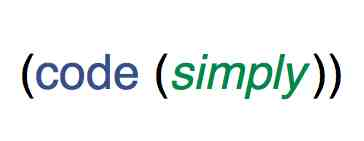
\includegraphics[height=0.5cm]{logo.pdf}}
\end{verbatim}

  Currently, the effect of this command is just to setup the |logo| template. However, a more sophisticated effect might be implemented in the future.

  \articlenote
  This command has no effect.

  \begin{element}{logo}\yes\yes\yes
    This template is used to render the logo.
  \end{element}

  The following insert can be used to insert a logo somewhere:
  \begin{itemize}
    \iteminsert{\insertlogo}
    inserts the logo at the current position. This command has the same effect as |\usebeamertemplate*{logo}|.
  \end{itemize}
\end{command}

\subsubsection{The Frame Title}

The frame title is shown prominently at the top of the frame and can be specified with the following command:

\begin{command}{\frametitle\sarg{overlay specification}\oarg{short frame title}\marg{frame title text}}
  You should end the \meta{frame title text} with a period, if the title is a proper sentence. Otherwise, there should not be a period. The \meta{short frame title} is normally not shown, but it's available via the |\insertshortframetitle| command. The \meta{overlay specification} is mostly useful for suppressing the frame title in |article| mode.

  \example
\begin{verbatim}
\begin{frame}
  \frametitle{A Frame Title is Important.}
  \framesubtitle{Subtitles are not so important.}

  Frame contents.
\end{frame}
\end{verbatim}

  If you are using the |allowframebreaks| option with the current frame, a continuation text (like ``(cont.)'' or something similar, depending on the template |frametitle continuation|) is automatically added to the \meta{frame title text} at the end, separated with a space.

  \beamernote
  The frame title is not typeset immediately when the command |\frametitle| is encountered. Rather, the argument of the command is stored internally and the frame title is only typeset when the complete frame has been read. This gives you access to both the \meta{frame title text} and to the \meta{subframe title text} that is possibly introduced using the |\framesubtitle| command.

  \articlenote
  By default, this command creates a new paragraph in |article| mode, entitled \meta{frame title text}. Using the \meta{overlay specification} makes it easy to suppress a frame title once in a while. If you generally wish to suppress \emph{all} frame titles in |article| mode, say |\setbeamertemplate<article>{frametitle}{}|.

  \begin{element}{frametitle}\yes\yes\yes
    \colorfontparents{titlelike}

    When the frame title and subtitle are to be typeset, this template is invoked with the \beamer-color and -font |frametitle| set. This template is \emph{not} invoked when the commands |\frametitle| or |\framesubtitle| are called. Rather, it is invoked when the whole frame has been completely read. Till then, the frame title and frame subtitle text are stored in a special place. This way, when the template is invoked, both inserts are setup correctly. The resulting \TeX-box is then magically put back to the top of the frame.

    \begin{templateoptions}
      \itemoption{default}{\oarg{alignment}}
      The frame is typeset using the \beamer-color |frametitle| and the \beamer-font |frametitle|. The subtitle is put below using the color and font |framesubtitle|. If the color |frametitle| has a background, a background bar stretching the whole frame width is put behind the title. A background color of the subtitle is ignored. The \meta{alignment} is passed on to the |beamercolorbox| environment. In particular, useful options are |left|, |center|, and |right|. As a special case, the |right| option causes the left border of the frame title to be somewhat larger than normal so that the frame title is more in the middle of the frame.

      \itemoption{shadow theme}{}
      This option is available if the outer theme |shadow| is loaded. It draws the frame title on top of a horizontal shading between the background colors of |frametitle| and |frametitle right|. A subtitle is, if present, also put on this bar. Below the bar, a ``shadow'' is drawn.

      \itemoption{sidebar theme}{}
      This option is available if the outer theme |sidebar| is loaded and if the headline height is not set to 0pt (which can be done using an option of the |sidebar| theme). With this option, the frame title is put inside a rectangular area that is part of the headline (some ``negative space'' is used to raise the frame title into this area). The background of the color |frametitle| is not used, this is the job of the headline template in this case.

      \itemoption{smoothbars theme}{}
      This option is available if the outer theme |smoothbars| is loaded. It typesets the frame title on a colored bar with the background color of |frametitle|. The top and bottom of the bar smoothly blend over to backgrounds above and below.

      \itemoption{smoothtree theme}{}
      Like |smoothbars theme|, only for the |smoothtree| theme.
    \end{templateoptions}

    The following commands are useful for this template:
    \begin{templateinserts}
      \iteminsert{\insertframetitle} yields the frame title.
      \iteminsert{\insertframesubtitle} yields the frame subtitle.
    \end{templateinserts}
  \end{element}
\end{command}


\begin{command}{\framesubtitle\sarg{overlay specification}\marg{frame subtitle text}}
  If present, a subtitle will be shown in a smaller font below the main title. Like the |\frametitle| command, this command can be given anywhere in the frame, since the frame title is actually typeset only when everything else has already been typeset.

  \example
\begin{verbatim}
\begin{frame}
  \frametitle<presentation>{Frame Title Should Be in Uppercase.}
  \framesubtitle{Subtitles can be in lowercase if they are full sentences.}

  Frame contents.
\end{frame}
\end{verbatim}

  \articlenote
  By default, the subtitle is not shown in any way in |article| mode.

  \begin{element}{framesubtitle}\no\yes\yes
    \colorfontparents{frametitle}
    This element provides a color and a font for the subtitle, but no template. It is the job of the |frametitle| template to also typeset the subtitle.
  \end{element}
\end{command}

Be default, all material for a slide is vertically centered. You can change this using the following class options:

\begin{classoption}{t}
  Place text of slides at the (vertical) top of the slides. This corresponds to a vertical ``flush.'' You can override this for individual frames using the |c| or |b| option.
\end{classoption}

\begin{classoption}{c}
  Place text of slides at the (vertical) center of the slides. This is the default. You can override this for individual frames using the |t| or |b| option.
\end{classoption}

\subsubsection{The Background}
\label{section-canvas}
\label{section-background}

Each frame has a \emph{background}, which---as the name suggests---is ``behind everything.'' The background is a surprisingly complex object: in \beamer, it consists of a \emph{background canvas} and the \emph{main background}.

The background canvas can be imagined as a large area on which everything (the main background and everything else) is painted on. By default, this canvas is a big rectangle filling the whole frame whose color is the background of the \beamer-color |background canvas|. Since this color inherits from |normal text|, by changing the background color of the normal text, you can change this color of the canvas.

\example
The following command changes the background color to a light red.
\begin{verbatim}
\setbeamercolor{normal text}{bg=red!20}
\end{verbatim}

The canvas need not be monochrome. Instead, you can install a shading or even make it transparent. Making it transparent is a good idea if you wish to include your slides in some other document.

\example
The following command makes the background canvas transparent:
\begin{verbatim}
\setbeamercolor{background canvas}{bg=}
\end{verbatim}

\begin{element}{background canvas}\yes\yes\yes
  \colorparents{normal text}
  The template is inserted ``behind everything.'' The template should typically be some \TeX\ commands that produce a rectangle of height |\paperheight| and width |\paperwidth|.

  \begin{templateoptions}
    \itemoption{default}{}
    installs a large rectangle with the background color. If the background is empty, the canvas is ``transparent.'' Since |background canvas| inherits from |normal text|, you can change the background of the \beamer-color |normal text| to change the color of the default canvas. However, to make the canvas transparent, only set the background of the canvas empty; leave the background of normal text white.

    \itemoption{vertical shading}{\oarg{color options}}
    installs a vertically shaded background. \emph{Use with care: Background shadings are often distracting!} The following \meta{color options} may be given:
    \begin{itemize}
      \item
      \declare{|top=|\meta{color}} specifies the color at the top of the page. By default, 25\% of the foreground of the \beamer-color |palette primary| is used.
      \item
      \declare{|bottom=|\meta{color}} specifies the color at the bottom of the page. By default, the background of |normal text| at the moment of invocation of this command is used.
      \item
      \declare{|middle=|\meta{color}} specifies the color for the middle of the page. Thus, if this option is given, the shading changes from the bottom color to this color and then to the top color.
      \item
      \declare{|midpoint=|\meta{factor}} specifies at which point of the page the middle color is used. A factor of |0| is the bottom of the page, a factor of |1| is the top. The default, which is |0.5| is in the middle.
    \end{itemize}
  \end{templateoptions}
\end{element}

The main background is drawn on top of the background canvas. It can be used to add, say, a grid to every frame or a big background picture or whatever. If you plan to use a PNG image as a background image, use one with an alpha channel to avoid potential problems with transparency in some PDF viewers.

\begin{element}{background}\yes\yes\yes
  \colorparents{background canvas}
  The template is inserted ``behind everything, but on top of the background canvas.'' Use it for pictures or grids or anything that does not necessarily fill the whole background. When this template is typeset, the \beamer-color and -font |background| will be setup.

  \begin{templateoptions}
    \itemoption{default}{} is empty.

    \itemoption{grid}{\oarg{grid options}}
    places a grid on the background. The following \meta{grid options} may be given:
    \begin{itemize}
      \item
      \declare{|step=|\meta{dimension}} specifies the distance between grid lines. The default is 0.5\,cm.
      \item
      \declare{|color=|\meta{color}} specifies the color of the grid lines. The default is 10\% foreground.
    \end{itemize}
  \end{templateoptions}
\end{element}


\subsection{Frame and Margin Sizes}

The size of a frame is actually the ``paper size'' of a \beamer\ presentation, and it is variable. By default, it amounts to 128\,mm by 96\,mm. The aspect ratio of this size is 4:3, which is exactly what most beamers offer these days. It is the job of the presentation program (like |acroread|, |xpdf|, |okular| or |evince|) to display the slides at full screen size. The main advantage of using a small ``paper size'' is that you can use all your normal fonts at their natural sizes. In particular, inserting a graphic with 11pt labels will result in reasonably sized labels during the presentation.

To change ``paper size'' and aspect ratio, you can use the following class options:

\begin{classoption}{aspectratio=2013}
  Sets aspect ratio to 20:13, and frame size to 140\,mm by 91\,mm.
\end{classoption}

\begin{classoption}{aspectratio=1610}
  Sets aspect ratio to 16:10, and frame size to 160\,mm by 100\,mm.
\end{classoption}

\begin{classoption}{aspectratio=169}
  Sets aspect ratio to 16:9, and frame size to 160\,mm by 90\,mm.
\end{classoption}

\begin{classoption}{aspectratio=149}
  Sets aspect ratio to 14:9, and frame size to 140\,mm by 90\,mm.
\end{classoption}

\begin{classoption}{aspectratio=141}
  Sets aspect ratio to 1.41:1, and frame size to 148.5\,mm by 105\,mm.
\end{classoption}

\begin{classoption}{aspectratio=54}
  Sets aspect ratio to 5:4, and frame size to 125\,mm by 100\,mm.
\end{classoption}

\begin{classoption}{aspectratio=43}
  The default aspect ratio and frame size. You need not specify this option.
\end{classoption}

\begin{classoption}{aspectratio=32}
  Sets aspect ratio to 3:2, and frame size to 135\,mm by 90\,mm.
\end{classoption}

\begin{classoption}{aspectratio=xxxx}
  Allows the user to set their own aspect ratio. For the height of the resulting frame, the default value of 96\,mm is used and the width will be calculated accordingly to match the desired aspect ratio.
  
  The custom aspect ratio allows for two to four digits and will be interpreted as shown in the following examples:
  \begin{itemize}
    \item two digits: |aspectratio=42| as 4:2
    \item three digits: |aspectratio=137| as 13:7 (e.g. always in landscape format)
    \item four digits: |aspectratio=1024| as 10:24
  \end{itemize} 
\end{classoption}

Aside from using these options, you should refrain from changing the ``paper size.'' However, you \emph{can} change the size of the left and right margins, which default to 1\,cm. To change them, you should use the following command:

\begin{command}{\setbeamersize\marg{options}}
  The following \meta{options} can be given:
  \begin{itemize}
  \item
    \declare{|text margin left=|\meta{\TeX\ dimension}} sets a new left margin. This excludes the left sidebar. Thus, it is the distance between the right edge of the left sidebar and the left edge of the text.
  \item
    \declare{|text margin right=|\meta{\TeX\ dimension}} sets a new right margin.
  \item
    \declare{|sidebar width left=|\meta{\TeX\ dimension}} sets the size of the left sidebar. Currently, this command should be given \emph{before} a shading is installed for the sidebar canvas.
  \item
    \declare{|sidebar width right=|\meta{\TeX\ dimension}} sets the size of the right sidebar.
  \item
    \declare{|description width=|\meta{\TeX\ dimension}} sets the default width of description labels, see Section~\ref{section-descriptions}.
  \item
    \declare{|description width of=|\meta{text}} sets the default width of description labels to the width of the \meta{text}, see Section~\ref{section-descriptions}.
  \item
    \declare{|mini frame size=|\meta{\TeX\ dimension}} sets the size of mini frames in a navigation bar. When two mini frame icons are shown alongside each other, their left end points are \meta{\TeX\ dimension} far apart.
  \item
    \declare{|mini frame offset=|\meta{\TeX\ dimension}} set an additional vertical offset that is added to the mini frame size when arranging mini frames vertically.
  \end{itemize}

  \articlenote
  This command has no effect in |article| mode.
\end{command}


\subsection{Restricting the Slides of a Frame}
\label{section-restriction}

The number of slides in a frame is automatically calculated. If the largest number mentioned in any overlay specification inside the frame is 4, four slides are introduced (despite the fact that a specification like |<4->| might suggest that more than four slides would be possible).

You can also specify the number of slides in the frame ``by hand.'' To do so, you pass an overlay specification to the |\frame| command. The frame will contain only the slides specified in this argument. Consider the following example.

\begin{verbatim}
\begin{frame}<1-2,4->
  This is slide number \only<1>{1}\only<2>{2}\only<3>{3}%
  \only<4>{4}\only<5>{5}.
\end{frame}
\end{verbatim}

This command will create a frame containing four slides. The first will contain the text ``This is slide number~1,'' the second ``This is slide number~2,'' the third ``This is slide number~4,'' and the fourth ``This is slide number~5.''

A useful specification is just |<0>|, which causes the frame to have no slides at all. For example, |\begin{frame}<handout:0>| causes the frame to be suppressed in the handout version, but to be shown normally in all other versions. Another useful specification is |<beamer>|, which causes the frame to be shown normally in |beamer| mode, but to be suppressed in all other versions.

Frames which are hidden with |<0>| behave like the |noframenumbering| option and will not be counted for the number of frames (this only applies if no mode is specified, e.g. not for |<all:0>|). 
